\section{Data Handling}\label{sec:data_handling}
The data handling occurring within \texttt{fmi2DoStep} of EDB FMU is described
below.
All values of messages with time stamps (converted to simulation time) within the
time interval $]currentSimulationTime,currentSimulationTime + simulationStepSize]$
overrides the current state of values in the received order, thus using
zero-order hold. This depends on the Data Middleware Node providing the data
order by time, as mentioned in \cref{sec:intro}.

An example is given in \cref{fig:data-handling-dostep}.
First, \texttt{message x} is received and overwrites the value of \texttt{a} in the EDB FMU state.\\
Afterwards, \texttt{message y} is received and overwrites the value of \texttt{b} in
the EDB FMU state.\\
Lastly, \texttt{message z} is received and overwrites the value of
\texttt{a} in the EDB FMU state. \\
The example above implies that the value of \texttt{a} in \texttt{message x}  is never
outputted from the EDB FMU, since it has been overwritten by the value of
\texttt{a} in \texttt{message z} within the same \texttt{fmi2DoStep} execution.

\begin{figure}[htb]
  \centering
  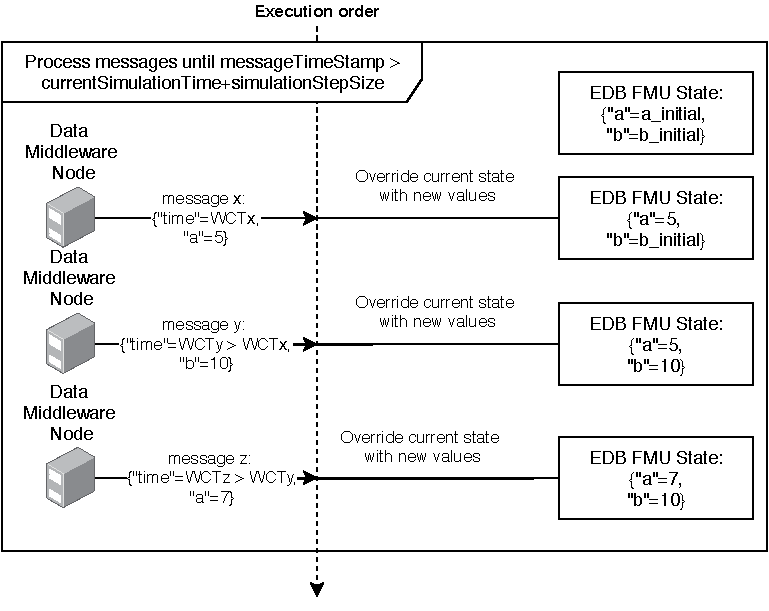
\includegraphics[width=\textwidth]{figures/datahandling.pdf}
  \caption{Data Handling in \texttt{fmi2DoStep}}
  \label{fig:data-handling-dostep}
\end{figure}

%%% Local Variables:
%%% mode: latex
%%% TeX-master: "../rabbitmq-fmu"
%%% End:
